  \documentclass[a4j,twocolumn]{jsarticle}
  \usepackage[dvipdfmx]{graphicx}
  \usepackage{url}

  \setlength{\textheight}{275mm}
  \headheight 5mm
  \topmargin -30mm
  \textwidth 185mm
  \oddsidemargin -15mm
  \evensidemargin -15mm
  \pagestyle{empty}


  \begin{document}

  \title{デジタル版しおりの開発}
  \author{情報科学科 \hspace{5mm} 37022463 \hspace{5mm} 西谷研究室 山本果音}
  \date{}

  \maketitle


\section{序論}
\label{sec:org6b99acf}
修学旅行などにおいて,参加者に対して事前に配布されるしおりは,旅程の把握や所持品の確認,集合時間の共有などを目的とした重要な情報媒体である.
近年では,紙媒体に代わりスマートフォンなどを用いて旅行情報を閲覧・共有するニーズが高まっており,これに応える形で旅しお[1]などのWebサービスが登場している.
しかし,旅行のプランニング用途で使用する場合,以下のような課題が存在する.
\begin{enumerate}
\item 図1のとおり,履歴には作成日・更新日が表示される一方で,旅行日付が時系列で整理されておらず,旅行の実施状況が視覚的に困難である.
\item 作成済みの旅行準備に対して旅行名や説明文のキーワードで検索する機能が存在しないため,過去の旅行記録を振り返る際に,スクロール操作によって目的のしおりを探す必要があり,利便性に欠ける.
\item 地図が表示されないため,目的地が視覚的に理解しにくい.
\end{enumerate}
結果として,利用者は外部ツールや手作業によって不足機能を補う必要があり,利便性や効率性に課題が残る.
そこで本研究では,旅行の予定管理だけでなく,旅行後の記録整理にも活用できる「デジタル版しおり」として機能する旅行プランニングアプリの開発を目指す.



\begin{figure}[htbp]
\centering
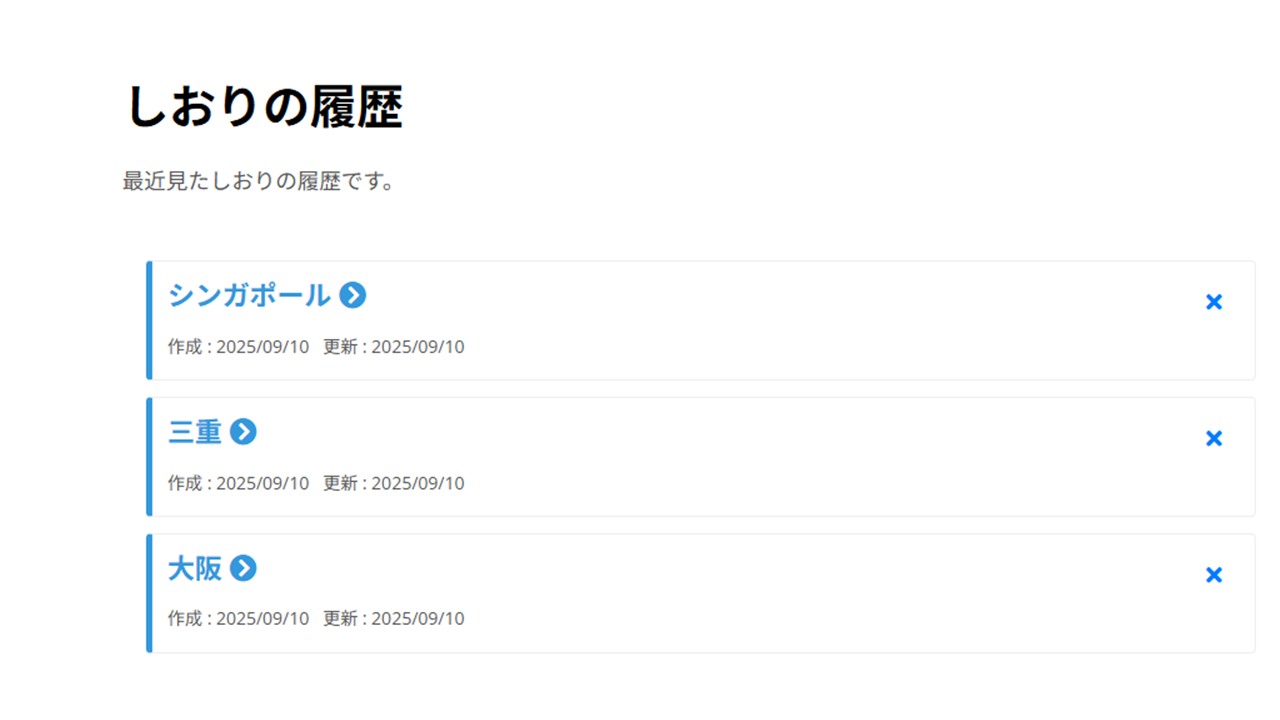
\includegraphics[width=7cm]{./figs/rireki1.png}
\caption{\label{fig:org4abda21}旅しおで作成したしおりの履歴表示画面.}
\end{figure}


\section{開発手法}
\label{sec:orge4e412a}
開発環境としてDjango[2]を選定した.
Djangoは、PythonベースのWebフレームワークである.
Djangoの利点は以下の2つである[3].
\begin{enumerate}
\item django-admin startproject コマンドにより,必要なファイルやフォルダが一式自動で作成されるため,迅速な開発が可能.
\item Djangoが提供するModelForm機能により,フォーム作成が容易にできる.
\item セキュリティ対策を実装しなくても,Djangoというフレームワーク自体が標準で安全性を確保する仕組みを備えているため安全である.
\end{enumerate}
また開発はPython, HTML, JavaScript, CSSを使用し、UIライブラリとしてはBootstrapを用いて開発を行った.


\section{結果}
\label{sec:orgdfbbe2d}
今回開発したWebアプリは,以下のような動作を行う.

\begin{enumerate}
\item 登録された旅行期間に基づき,図2のとおり「完了した旅行」「旅行中」「予定の旅行」「期間未設定」のいずれに該当するかを判定し,色分けして表示することで,旅行の状態を視覚的に把握しやすくする.
\item 旅行名や説明文に含まれるキーワードで検索が可能であり,目的の旅行をすばやく見つけることができる.
\end{enumerate}
これにより,過去の履歴と今後の予定を視覚的に整理することができるため,ユーザーが「どこに行ったか」「次にどこへ行くか」を一目で認識できるようになった.
また,ユーザーの記憶が曖昧な場合でも関連するキーワードから目的の旅行を容易に特定することが可能となり,再訪計画にも活用が可能になった.

\begin{figure}[htbp]
\centering
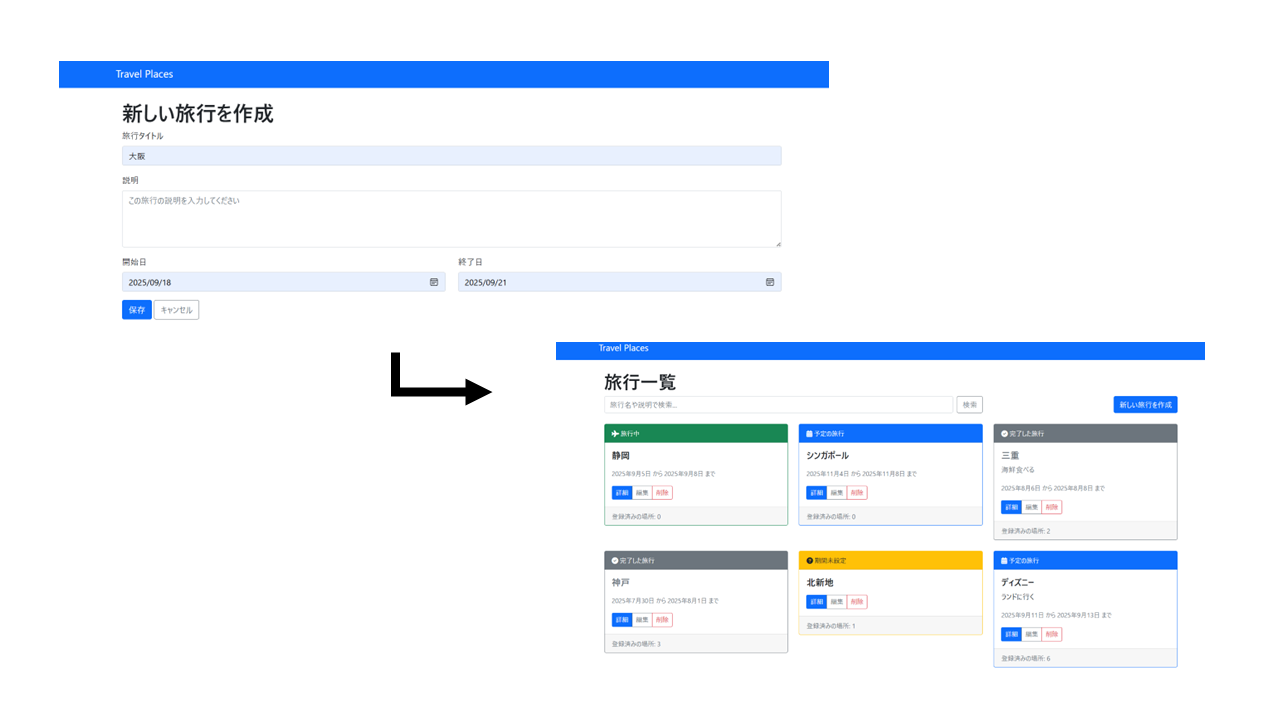
\includegraphics[width=10cm]{./figs/trip1.png}
\caption{\label{fig:org02cd3fb}旅行日付に基づく時系列判定と色分けによる視覚的管理を行ったときの画面.}
\end{figure}


\section{今後の課題}
\label{sec:orgf534867}
今回は,旅行日付に基づく色分け表示,キーワード検索機能を開発した.
今後は,旅行先の地理的な位置関係を視覚的に把握できるようにする地図の表示,旅行準備の漏れを防ぐための所持品チェックリスト機能や,日程に応じて柔軟に観光訪問順を変更できる入れ替え機能の開発を予定している.
これにより,地理情報・所持品の準備・当日の柔軟性といった複数の観点から旅行準備計画を支援することで,ユーザーの意図に沿った旅行体験が可能となる.



\small\setlength\baselineskip{10pt}
\begin{thebibliography}{9}

\bibitem{旅しお} 旅しお,\url{https://tabisio.com/},(2025/09/05 accessed).
\bibitem{Django}Djangoドキュメント,\url{https://docs.djangoproject.com/ja/5.1/topics/},(2025/09/05 accessed).
\bibitem{Django}Django,\url{https://www.djangoproject.com/},(2025/09/05 accessed).
\end{thebibliography}
\end{document}
